\section{Lösungskonzept}
Dieses Kapitel beinhaltet die Beschreibung der Architektur und wichtiger Komponenten. Die eingesetzten Technologien und genauen Implementationsdetails stehen im Hintergrund und werden im Kapitel 4 aufgegriffen. Ausserdem wird erklärt, welches Plattform verwendet wird und warum sie ausgewählt wurde.

\subsection{Evaluation der Plattform}
Anhand der Marktsituation und den funkionalen Anforderungen haben wir die Vor- und Nachteile der jeweiligen Plattformen miteinander verglichen und dabei darauf geachtet, welche Kriterien für unsere Lösung von Bedeutung sind.

Wichtige Kriterien:
\begin{itemize}
	\item Nachträgliche Installation möglich
	\item Beliebige Szenarien realisierbar
	\item Herstellerunabhängige Komponenten
	\item Erfüllung der Anforderungen F01 - F05
\end{itemize}

Vernachlässigbare Kriterien:
\begin{itemize}
	\item Optisch ansprechende Integration
	\item Installation ohne Fachkenntnisse
\end{itemize}

\subsubsection{Ergebnis: openHAB} 
Mit openHAB haben wir eine Plattform gefunden, die allen wichtigen Kriterien entspricht und zudem kostenlos ist. Da wir openHAB sofort auf unseren Notebooks installieren konnten, war es sehr einfach zu beurteilen, ob die Plattform auch in der Praxis unsere Anforderungen erfüllt. Die mitgelieferte Demo-Konfiguration beinhaltete bereits viele anschauliche Beispiele, die später als Vorlage für unsere eigenen Anwendungsfälle dienen können. 

\textbf{Erfüllung der funktionalen Anforderungen} \\
\textit{F01 - F02:} Über sogenannte Items können Sensoren und Aktoren virtuell und genügend abstrakt definiert werden. Der OSGi EventBus von openHAB ermöglicht den Transport von Events und Commands zwischen Items und der Zentrale (OpenHAB Runtime). Bindings mappen die Items auf tatsächliche Sensoren und Aktoren.

\textit{F03:} OpenHAB kann den Verkehr auf dem EventBus über verschiedene Wege auf externen Systemen protokollieren. Zu unserem Zweck eignet sich das MQTT Persistence Modul.

\textit{F04:} Über die Rule Engine von openHAB können Regeln mit Hilfe einer Java-ähnlichen DSL beschrieben werden. Regeln werden bei gewissen Events auf dem EventBus ausgeführt. Die DLS erlaubt den Zugriff auf den Zustand von Items und kann auch Commands an Items und somit an Aktoren senden.

\textit{F05:} Ein RESTful API bietet umfassenden Zugriff auf die openHAB Runtime. Über sogenannte Sitemaps können deskriptive User Interfaces automatisch generiert werden.



\textbf{Nachteile} \\
Ein Nachteil an openHAB ist, dass die Dokumentation grosse Lücken aufweist. Zwar sind die Konzepte leichte verständlich, jedoch fehlen Detailangaben zur DSL und genauen Konfigurationssyntax. Aus diesem Grund müssen oft Beispiele analysiert oder Benutzerforen zu Rate gezogen werden.

\subsection{Evaluation der Hardware}
Nachdem wir openHAB als Plattform bestimmt haben konnten wir die Hardware für die Sensoren und Aktoren aussuchen. Dafür haben wir uns an den Vorgaben L02 - L06 aus Abschnitt 2.2.2 orientiert. Durch die Vielzahl an Protokollen, die durch openHAB unterstützt werden, hatten wir genügend Auswahl an Hardware von unterschiedlichen Herstellern. OpenHAB selbst läuft auf einem Raspberry Pi B+.

\textit{L02:} Als Überwachungskamera haben wir die Edimax IC-3115W Netzwerkkamera ausgesucht. Sie ist mit einem Preis von weniger als 50 Euro relativ günstig und über das HTTP Binding von openHAB kompatibel.

\textit{L03:} Beim Fensterkontaktsensor war uns ein kabelloses Modell wichtig, das unkompliziert montiert werden kann. Aus diesem Grund haben wir uns für den optischen Fensterkontakt HM-Sec-Sco von eQ-3 HomeMatic entschieden. Der Fensterkontakt erfordert jedoch eine Zentrale, die separat bestellt werden musste. Für HomeMatic existiert ein Binding seitens openHAB.

\textit{L04:} Der Funk Bewegungsmelder HM-Sec-MDIR-2, ebenfalls von eQ-3 HomeMatic, benutzt die gleiche Zentrale wie der Fensterkontaktsensor und ist für den Indoorgebrauch ausgelegt.

\textit{L05:} Das Philips Hue Lux Starterkit beinhaltet zwei dimmbare LED-Birnen und eine Zentrale, die ans lokale Netzwerk angeschlossen werden muss. Ein openHAB Binding für Philips Hue ist vorhanden.

\textit{L06:} Da wir durch den Fensterkontakt und den Bewegungsmelder schon eine HomeMatic Zentrale besitzen, liegt es nahe auch die Funksteckdose von diesem Hersteller zu verwenden.

\subsection{MQTT}
\subsubsection{Broker Evaluation}
Für die Evaluation des Brokers haben wir eine List mit unseren Anforderungen erstellt: 

\begin{enumerate}
	\item Open Source/Freeware
	\item SSL TLS Verschlüsselung
	\item Benutzername \& Passwort Authentifizierung
	\item High throughput, Low latency
	\item Cloud Ready
	\item Einfache Installation
	\item Qualit of Service Level: Exactly once
	\item Last Will unterstützung (Message, die gesendet wird, wenn der Client die Verbindung schliesst)
\end{enumerate}

\textbf{HiveMQ (\url{http://www.hivemq.com})} \\
HiveMQ ist ein proprietärer MQTT-Broker und erfüllt alle unsere Kriterien bis auf das erste Kriterium. Jeder Gebrauch des Brokers muss bezahlt werden, siehe: \url{http://www.hivemq.com/pricing/}.

\textbf{Mosquitto (\url{http://eclipse.org/mosquitto/})}\\
Mosquitto ist ein Open Source Broker, dessen Projekt von Roger Light im Jahr 2010 auf die Beine gestellt wurde. Seit der Version 1.4 läuft das Projekt unter der Eclipse Foundation. \\
Die aktuelle Implementation benötigt lediglich 120kB Speicherplatz und 3MB RAM bei 1000 verbundenen Clients. Ein Belastungstest von 100'000 Clients erzielte erfolgreiche und zufriedenstellende Resultate.
Alle anderen Kriterien werden ebenfalls erfüllt.

\textbf{CloudMQTT} \\
CloudMQTT unterscheidet sich von den anderen Brokern, da dieser nicht selbst betrieben werden kann. Das bedeutet, man erstellt bei CloudMQTT eine Instanz und kann denn neu erstellten Broke über verschiedene APIs ansteuern. \\
Der Anbieter stellt verschiedene Preispläne zur Verfügung (\url{http://www.cloudmqtt.com/plans.html}). Ab 10 Verbindungen bzw. 10Kbit/s Bandbreite muss für die Leistung bezahlt werden. \\
Ob TLS SSL Verschlüsselung unterstützt wird, ist in der spärlichen Dokumentation nicht ersichtlich.

\textbf{Fazit} \\
Aufgrund der gesammelten Daten der drei Produkte wurde entschieden, Mosquitto einzusetzen. Es ist das einzige Produkt, welches alle unsere Kriterien erfüllt. Da dieses Projekt durch die Eclipse Foundation unterstützt wird, besteht die Hoffung, dass die Zusammenarbeit mit openHAB unterstützt bzw. miteinbezogen wurde.

\subsubsection{Client-Library}
In unserem Systemaufbau wird es zwei MQTT-Clients geben. Einerseits durch das openHAB-Binding, da die Events auf dem EventBus über MQTT in die Azure Cloud gesendet werden soll. Andererseits wird in der Cloud eine Worker Role diese Events konsumieren und persistieren. \\
Das Binding von openHAB besteht bereits, daher muss nur noch eine Client-Implementation für C\# gesuchtwerden. Nach kurzer Rechereche scheint die «M2Mqtt» Library sehr verbreitet zu sein. \\
Durch aufsetzen eines Prototyps konnte die benötigte Funktionalität erfasst werden. Sie erfüllt alle Kriterien, die auch an den Broker gestellt wurden.

\subsection{Sicherheit}
In unserem Szenario, Einbruchschutz, ist das Thema Sicherheit sehr wichtig. Daher lohnt es sich dazu  Gedanken zu machen. Man kann das System grob in drei Bereiche einteilen, an denen ein Angriff angesetzt werden kann:
\begin{itemize}
	\item Cloud
	\item Android App
	\item Systemaufbau mit Sensoren/Aktoren
	\item Kommunikation der HomeMatic Komponenten
\end{itemize}

\subsubsection{Cloud}
Die Angriffsfläche in der Cloud ist ziemlich eingeschränkt. Sicherheitsrelevante Aspekte sind der Broker und die persistierten Daten im Storage. Zugriff auf diese Ressourcen erhält man über verschiedene Wege. Einerseits über das Management Web-Interface von Microsoft Azure oder über ein Connection-String. Durch die Verwendung eines Connection Strings für den Verbindungsaufbau zum Storage kein Benutzername bzw. Passwort mitgegeben werden.

Zugriff auf diese Ressourcen haben nur authorisierte Personen die ein entsprechendes Microsoft Konto besitzen und auf die Subscription zugelassen werden. Eine vernünftige Attack kann daher nur durch das Hijacken eines Accounts gefahren werden. Als Gegenmassnahme müssen ausreichend sichere Passwörter auf den persönlichen Konten gesetzt werden. Das liegt in der Verantwortung der einzelnen Personen, die auf diese Subscription Zugriff besitzen.

Auf den Storage kann ausser der Management-Oberfläche auch über ein Connection-String zugegriffen werden. Dieser String kann nur über die Management-Oberfläche eingesehen werden und ist daher sicher versteckt. Weiter könnte der Connection String aus dem Source-Code der Worker Role gelesen werden, da er dort für den Verbindungsaufbau zum Storage verwendet wird. Diese Worker Role und deren Source-Code befindet sich innerhalb der Cloud und ist somit auch gegen ein Eindringen gesichert. \\

\subsubsection{Android App}
Über das Android App kann das ganze System manipuliert werden. Daher stellt dies ein grosses Sicherheits-Risiko dar. Gesichtert wird das App durch Eingabe von Benutzerdaten, um auf die RESTful-API des openHAB zuzugreifen. \\
Auch hier wird die Person, die das App verwendet zur Verantwortung gezogen, um das Smartphone durch ein sicheres Passwort zu schützen.

\subsubsection{Systemaufbau mit Sensoren/Aktoren}
Wenn sich die angreifende Person bereits im Haus befindet,hat sie die entsprechenden Alarme bereits ausgelöst und wurde durch die Webcam aufgenommen. \\
Für dieses Szenario ist das grösste Risiko, dass die Person die Videoüberwachung bemerkt und aus diesem Grund das Raspberry Pi zerstört bzw. mitnimmt. Um die aufgezeichneten Daten zu sichern, werden die von der Kamera erzeugten Bilder über MQTT im Cloud-Storage abgelegt. Auch wenn das Raspberry Pi zerstört wird, sind die Bilder nun gesichert und können im Nachhinein vom Storage heruntergeladen werden.

\subsubsection{HomeMatic Kommunikation}
Da die HomeMatic Komponenten untereinander drahtlos kommunizieren besteht hier ebenfalls die Gefahr einer Attacke. HomeMatic setzt für die Übertragung auf den Funkstandard BidCos. Diese Standard sieht vor, dass das 868 MHz Band verwendet wird. Im Vergleich zu 2.4 GHz besitzt man so eine grösse Reichweite und die Gefahr von Interferenz durch andere Funkgeräte ist sehr minim.\\
Bezüglich Sicherheit sieht der Standard lediglich vor, die übertragenen Daten durch XOR-Operationen unleserlich zu machen. HomeMatic hat daher bei der Implentierung dieses Stanards die Verschlüsselung durch AES-128 verstärkt. Der zur Verschlüsselung verwendete Key ist in der Zentrale hinterlegt und kann bei Bedarf geändert werden.


\subsubsection{Fazit}
Wie aus den Ausführungen zur Sicherheit ersichtlich ist, können alle technischen Sicherheits-Risiken abgedeckt werden. Die grösste Schwachstellt ist jeweils der Mensch, der durch Social-Engineering-Techniken manipuliert werden kann und so Zugriff auf das Android App gewährt.

\subsection{Allgemeine Systemsicht}
Anhand der Problembeschreibung wurde ein Plan erarbeitet, der das ganze System verständlich beschreibt. Abbildung \ref{fig:systemView} stellt die wichtigsten Komponenten und Entitäten aus der Problemdomäne in gegenseitiger Beziehung dar.

\begin{figure}[h!]
	\centering
		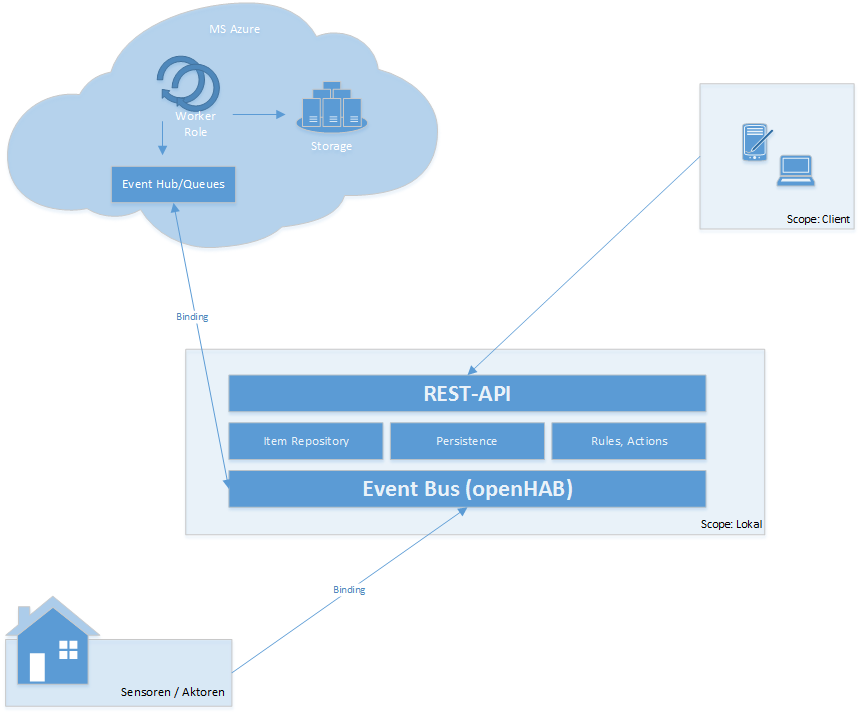
\includegraphics[scale=0.55]{report/img/systemuebersicht}
	\caption{Systemübersicht}
	\label{fig:systemView}
\end{figure}

\pagebreak